% ref: https://tikz.net/fast-fourier-transform/
% author: Alexandros Tsagkaropoulos

\documentclass{standalone}

\usepackage{tikz}
\usetikzlibrary{calc, shapes.multipart}

\def\nodeminheight{20pt}

\newcommand{\butterflyop}[8]{
% Circle
\coordinate (stage#1#2_points#3#4_tmp_west) at ($(stage_#1.#3 east)!0.5!(stage_#1.#4 east)$); 
\coordinate (stage#1#2_points#3#4_tmp_east) at ($(stage_#2.#3 west)!0.5!(stage_#2.#4 west)$); 
\node[draw, circle, fill=#8, inner sep = 2pt] (stage#1#2_points#3#4) at 
									 ($(stage#1#2_points#3#4_tmp_west)!#6!(stage#1#2_points#3#4_tmp_east)$) {}; 
% Breakpoints
\coordinate (stage#1#2_points_#3#4_up_0) at ($(stage_#1.#3 east)!#5!(stage_#2.#3 west)$);
\coordinate (stage#1#2_points_#3#4_up_1) at ($(stage_#1.#3 east)!#7!(stage_#2.#3 west)$);

\coordinate (stage#1#2_points_#3#4_down_0) at ($(stage_#1.#4 east)!#5!(stage_#2.#4 west)$);
\coordinate (stage#1#2_points_#3#4_down_1) at ($(stage_#1.#4 east)!#7!(stage_#2.#4 west)$);

% Connections
\draw (stage_#1.#3 east) -- 
	  (stage#1#2_points_#3#4_up_0) -- (stage#1#2_points#3#4) -- (stage#1#2_points_#3#4_up_1) -- 
	  (stage_#2.#3 west);
\draw (stage_#1.#4 east) -- 
	  (stage#1#2_points_#3#4_down_0) -- (stage#1#2_points#3#4) -- (stage#1#2_points_#3#4_down_1) -- 
	  (stage_#2.#4 west);
}

\begin{document}
	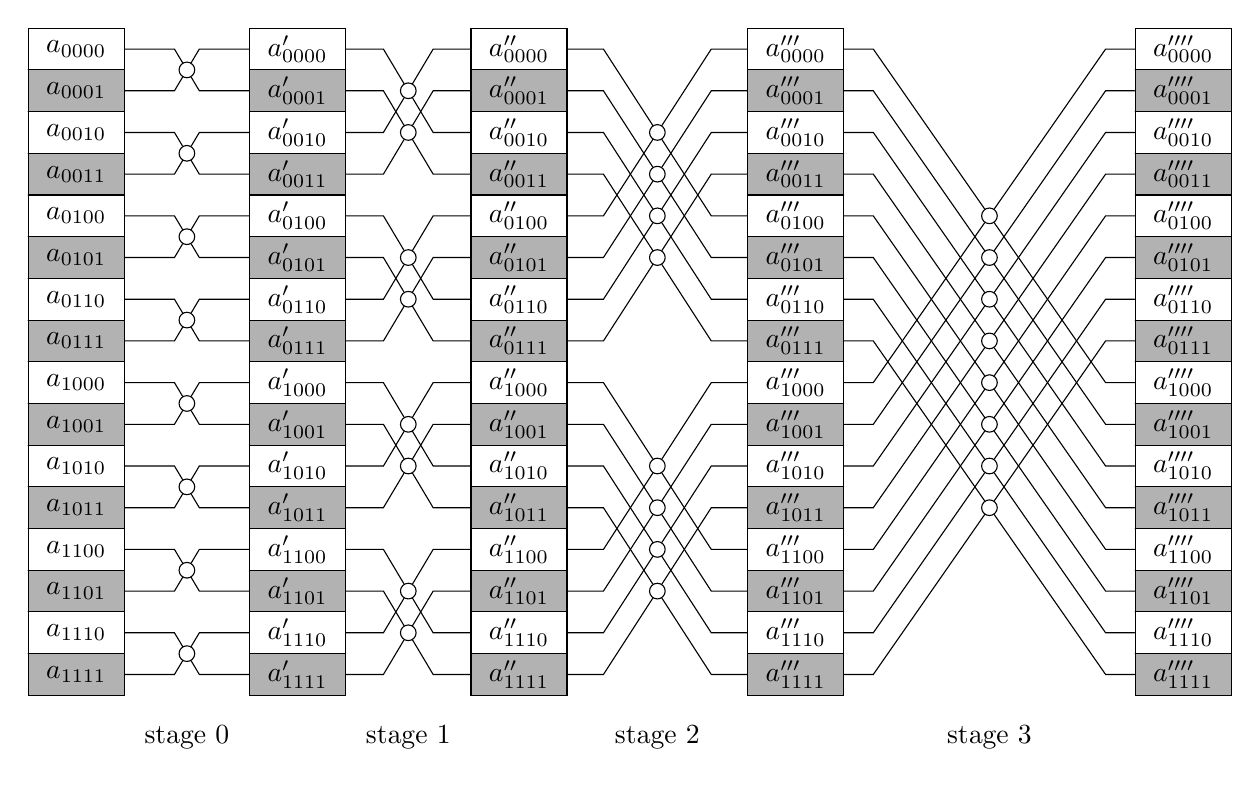
\begin{tikzpicture}[line cap = round]
		% Stage 0
		\node
			[
				draw, 
				rectangle split, 
				rectangle split parts = 16, 
				anchor = center,
				minimum height = \nodeminheight,
				rectangle split part fill = 
					{
						white, 
						gray!60,
						white, 
						gray!60,
						white, 
						gray!60,
						white, 
						gray!60,
						white, 
						gray!60,
						white, 
						gray!60,
						white, 
						gray!60,
						white, 
						gray!60,
					}
			] (stage_0) 
			{
				\parbox[c][8pt][c]{28pt}{\centering $a_{0000}$} \nodepart{two}
				\parbox[c][8pt][c]{28pt}{\centering $a_{0001}$} \nodepart{three}
				\parbox[c][8pt][c]{28pt}{\centering $a_{0010}$} \nodepart{four}
				\parbox[c][8pt][c]{28pt}{\centering $a_{0011}$} \nodepart{five}
				\parbox[c][8pt][c]{28pt}{\centering $a_{0100}$} \nodepart{six}
				\parbox[c][8pt][c]{28pt}{\centering $a_{0101}$} \nodepart{seven}
				\parbox[c][8pt][c]{28pt}{\centering $a_{0110}$} \nodepart{eight}
				\parbox[c][8pt][c]{28pt}{\centering $a_{0111}$} \nodepart{nine}
				\parbox[c][8pt][c]{28pt}{\centering $a_{1000}$} \nodepart{ten}
				\parbox[c][8pt][c]{28pt}{\centering $a_{1001}$} \nodepart{eleven}
				\parbox[c][8pt][c]{28pt}{\centering $a_{1010}$} \nodepart{twelve}
				\parbox[c][8pt][c]{28pt}{\centering $a_{1011}$} \nodepart{thirteen}
				\parbox[c][8pt][c]{28pt}{\centering $a_{1100}$} \nodepart{fourteen}
				\parbox[c][8pt][c]{28pt}{\centering $a_{1101}$} \nodepart{fifteen}
				\parbox[c][8pt][c]{28pt}{\centering $a_{1110}$} \nodepart{sixteen}
				\parbox[c][8pt][c]{28pt}{\centering $a_{1111}$}
			};

		% Stage 1
		\node
			[
				draw, 
				xshift = 8em,
				rectangle split, 
				rectangle split parts = 16, 
				anchor = center,
				minimum height = \nodeminheight,
				rectangle split part fill = 
					{
						white, 
						gray!60,
						white, 
						gray!60,
						white, 
						gray!60,
						white, 
						gray!60,
						white, 
						gray!60,
						white, 
						gray!60,
						white, 
						gray!60,
						white, 
						gray!60,
					}
			] (stage_1) 
			{
				\parbox[c][8pt][c]{28pt}{\centering $a'_{0000}$} \nodepart{two}
				\parbox[c][8pt][c]{28pt}{\centering $a'_{0001}$} \nodepart{three}
				\parbox[c][8pt][c]{28pt}{\centering $a'_{0010}$} \nodepart{four}
				\parbox[c][8pt][c]{28pt}{\centering $a'_{0011}$} \nodepart{five}
				\parbox[c][8pt][c]{28pt}{\centering $a'_{0100}$} \nodepart{six}
				\parbox[c][8pt][c]{28pt}{\centering $a'_{0101}$} \nodepart{seven}
				\parbox[c][8pt][c]{28pt}{\centering $a'_{0110}$} \nodepart{eight}
				\parbox[c][8pt][c]{28pt}{\centering $a'_{0111}$} \nodepart{nine}
				\parbox[c][8pt][c]{28pt}{\centering $a'_{1000}$} \nodepart{ten}
				\parbox[c][8pt][c]{28pt}{\centering $a'_{1001}$} \nodepart{eleven}
				\parbox[c][8pt][c]{28pt}{\centering $a'_{1010}$} \nodepart{twelve}
				\parbox[c][8pt][c]{28pt}{\centering $a'_{1011}$} \nodepart{thirteen}
				\parbox[c][8pt][c]{28pt}{\centering $a'_{1100}$} \nodepart{fourteen}
				\parbox[c][8pt][c]{28pt}{\centering $a'_{1101}$} \nodepart{fifteen}
				\parbox[c][8pt][c]{28pt}{\centering $a'_{1110}$} \nodepart{sixteen}
				\parbox[c][8pt][c]{28pt}{\centering $a'_{1111}$}			};
			
		% Stage 2
		\node
			[
				draw, 
				xshift = 16em,
				rectangle split, 
				rectangle split parts = 16, 
				anchor = center,
				minimum height = \nodeminheight,
				rectangle split part fill = 
					{
						white, 
						gray!60,
						white, 
						gray!60,
						white, 
						gray!60,
						white, 
						gray!60,
						white, 
						gray!60,
						white, 
						gray!60,
						white, 
						gray!60,
						white, 
						gray!60,
					}
			] (stage_2) 
			{
				\parbox[c][8pt][c]{28pt}{\centering $a''_{0000}$} \nodepart{two}
				\parbox[c][8pt][c]{28pt}{\centering $a''_{0001}$} \nodepart{three}
				\parbox[c][8pt][c]{28pt}{\centering $a''_{0010}$} \nodepart{four}
				\parbox[c][8pt][c]{28pt}{\centering $a''_{0011}$} \nodepart{five}
				\parbox[c][8pt][c]{28pt}{\centering $a''_{0100}$} \nodepart{six}
				\parbox[c][8pt][c]{28pt}{\centering $a''_{0101}$} \nodepart{seven}
				\parbox[c][8pt][c]{28pt}{\centering $a''_{0110}$} \nodepart{eight}
				\parbox[c][8pt][c]{28pt}{\centering $a''_{0111}$} \nodepart{nine}
				\parbox[c][8pt][c]{28pt}{\centering $a''_{1000}$} \nodepart{ten}
				\parbox[c][8pt][c]{28pt}{\centering $a''_{1001}$} \nodepart{eleven}
				\parbox[c][8pt][c]{28pt}{\centering $a''_{1010}$} \nodepart{twelve}
				\parbox[c][8pt][c]{28pt}{\centering $a''_{1011}$} \nodepart{thirteen}
				\parbox[c][8pt][c]{28pt}{\centering $a''_{1100}$} \nodepart{fourteen}
				\parbox[c][8pt][c]{28pt}{\centering $a''_{1101}$} \nodepart{fifteen}
				\parbox[c][8pt][c]{28pt}{\centering $a''_{1110}$} \nodepart{sixteen}
				\parbox[c][8pt][c]{28pt}{\centering $a''_{1111}$}		
	};

		% Stage 3
		\node
			[
				draw, 
				xshift = 26em,
				rectangle split, 
				rectangle split parts = 16, 
				anchor = center,
				minimum height = \nodeminheight,
				rectangle split part fill = 
					{
						white, 
						gray!60,
						white, 
						gray!60,
						white, 
						gray!60,
						white, 
						gray!60,
						white, 
						gray!60,
						white, 
						gray!60,
						white, 
						gray!60,
						white, 
						gray!60,
					}
			] (stage_3) 
			{
				\parbox[c][8pt][c]{28pt}{\centering $a'''_{0000}$} \nodepart{two}
				\parbox[c][8pt][c]{28pt}{\centering $a'''_{0001}$} \nodepart{three}
				\parbox[c][8pt][c]{28pt}{\centering $a'''_{0010}$} \nodepart{four}
				\parbox[c][8pt][c]{28pt}{\centering $a'''_{0011}$} \nodepart{five}
				\parbox[c][8pt][c]{28pt}{\centering $a'''_{0100}$} \nodepart{six}
				\parbox[c][8pt][c]{28pt}{\centering $a'''_{0101}$} \nodepart{seven}
				\parbox[c][8pt][c]{28pt}{\centering $a'''_{0110}$} \nodepart{eight}
				\parbox[c][8pt][c]{28pt}{\centering $a'''_{0111}$} \nodepart{nine}
				\parbox[c][8pt][c]{28pt}{\centering $a'''_{1000}$} \nodepart{ten}
				\parbox[c][8pt][c]{28pt}{\centering $a'''_{1001}$} \nodepart{eleven}
				\parbox[c][8pt][c]{28pt}{\centering $a'''_{1010}$} \nodepart{twelve}
				\parbox[c][8pt][c]{28pt}{\centering $a'''_{1011}$} \nodepart{thirteen}
				\parbox[c][8pt][c]{28pt}{\centering $a'''_{1100}$} \nodepart{fourteen}
				\parbox[c][8pt][c]{28pt}{\centering $a'''_{1101}$} \nodepart{fifteen}
				\parbox[c][8pt][c]{28pt}{\centering $a'''_{1110}$} \nodepart{sixteen}
				\parbox[c][8pt][c]{28pt}{\centering $a'''_{1111}$}
			};
			
		% Stage 4
		\node
			[
				draw, 
				xshift = 40em,
				rectangle split, 
				rectangle split parts = 16, 
				anchor = center,
				minimum height = \nodeminheight,
				rectangle split part fill = 
					{
						white, 
						gray!60,
						white, 
						gray!60,
						white, 
						gray!60,
						white, 
						gray!60,
						white, 
						gray!60,
						white, 
						gray!60,
						white, 
						gray!60,
						white, 
						gray!60,
					}
			] (stage_4) 
			{
				\parbox[c][8pt][c]{28pt}{\centering $a''''_{0000}$} \nodepart{two}
				\parbox[c][8pt][c]{28pt}{\centering $a''''_{0001}$} \nodepart{three}
				\parbox[c][8pt][c]{28pt}{\centering $a''''_{0010}$} \nodepart{four}
				\parbox[c][8pt][c]{28pt}{\centering $a''''_{0011}$} \nodepart{five}
				\parbox[c][8pt][c]{28pt}{\centering $a''''_{0100}$} \nodepart{six}
				\parbox[c][8pt][c]{28pt}{\centering $a''''_{0101}$} \nodepart{seven}
				\parbox[c][8pt][c]{28pt}{\centering $a''''_{0110}$} \nodepart{eight}
				\parbox[c][8pt][c]{28pt}{\centering $a''''_{0111}$} \nodepart{nine}
				\parbox[c][8pt][c]{28pt}{\centering $a''''_{1000}$} \nodepart{ten}
				\parbox[c][8pt][c]{28pt}{\centering $a''''_{1001}$} \nodepart{eleven}
				\parbox[c][8pt][c]{28pt}{\centering $a''''_{1010}$} \nodepart{twelve}
				\parbox[c][8pt][c]{28pt}{\centering $a''''_{1011}$} \nodepart{thirteen}
				\parbox[c][8pt][c]{28pt}{\centering $a''''_{1100}$} \nodepart{fourteen}
				\parbox[c][8pt][c]{28pt}{\centering $a''''_{1101}$} \nodepart{fifteen}
				\parbox[c][8pt][c]{28pt}{\centering $a''''_{1110}$} \nodepart{sixteen}
				\parbox[c][8pt][c]{28pt}{\centering $a''''_{1111}$}
			};
			
			% Network
			%% Stage_0 - Stage_1 Connections
			\butterflyop{0}{1}{one}{two}{0.4}{0.5}{0.6}{white}
			\butterflyop{0}{1}{three}{four}{0.4}{0.5}{0.6}{white}
			\butterflyop{0}{1}{five}{six}{0.4}{0.5}{0.6}{white}
			\butterflyop{0}{1}{seven}{eight}{0.4}{0.5}{0.6}{white}
			\butterflyop{0}{1}{nine}{ten}{0.4}{0.5}{0.6}{white}
			\butterflyop{0}{1}{eleven}{twelve}{0.4}{0.5}{0.6}{white}
			\butterflyop{0}{1}{thirteen}{fourteen}{0.4}{0.5}{0.6}{white}
			\butterflyop{0}{1}{fifteen}{sixteen}{0.4}{0.5}{0.6}{white}
			%% Stage_1 - Stage_2 Connections
			\butterflyop{1}{2}{one}{three}{0.3}{0.5}{0.7}{white}
			\butterflyop{1}{2}{two}{four}{0.3}{0.5}{0.7}{white}
			\butterflyop{1}{2}{five}{seven}{0.3}{0.5}{0.7}{white}
			\butterflyop{1}{2}{six}{eight}{0.3}{0.5}{0.7}{white}
			\butterflyop{1}{2}{nine}{eleven}{0.3}{0.5}{0.7}{white}
			\butterflyop{1}{2}{ten}{twelve}{0.3}{0.5}{0.7}{white}
			\butterflyop{1}{2}{thirteen}{fifteen}{0.3}{0.5}{0.7}{white}
			\butterflyop{1}{2}{fourteen}{sixteen}{0.3}{0.5}{0.7}{white}
			%% Stage_2 - Stage_3 Connections
			\butterflyop{2}{3}{one}{five}{0.2}{0.5}{0.8}{white}
			\butterflyop{2}{3}{two}{six}{0.2}{0.5}{0.8}{white}
			\butterflyop{2}{3}{three}{seven}{0.2}{0.5}{0.8}{white}
			\butterflyop{2}{3}{four}{eight}{0.2}{0.5}{0.8}{white}
			\butterflyop{2}{3}{nine}{thirteen}{0.2}{0.5}{0.8}{white}
			\butterflyop{2}{3}{ten}{fourteen}{0.2}{0.5}{0.8}{white}
			\butterflyop{2}{3}{eleven}{fifteen}{0.2}{0.5}{0.8}{white}
			\butterflyop{2}{3}{twelve}{sixteen}{0.2}{0.5}{0.8}{white}
			%% Stage_3 - Stage_4 Connections
			\butterflyop{3}{4}{one}{nine}{0.1}{0.5}{0.9}{white}
			\butterflyop{3}{4}{two}{ten}{0.1}{0.5}{0.9}{white}
			\butterflyop{3}{4}{three}{eleven}{0.1}{0.5}{0.9}{white}
			\butterflyop{3}{4}{four}{twelve}{0.1}{0.5}{0.9}{white}
			\butterflyop{3}{4}{five}{thirteen}{0.1}{0.5}{0.9}{white}
			\butterflyop{3}{4}{six}{fourteen}{0.1}{0.5}{0.9}{white}
			\butterflyop{3}{4}{seven}{fifteen}{0.1}{0.5}{0.9}{white}
			\butterflyop{3}{4}{eight}{sixteen}{0.1}{0.5}{0.9}{white}
			
			% Stages
			\node[yshift=-15pt] at ($(stage_0.south east)!0.5!(stage_1.south west)$) {stage 0};
			\node[yshift=-15pt] at ($(stage_1.south east)!0.5!(stage_2.south west)$) {stage 1};
			\node[yshift=-15pt] at ($(stage_2.south east)!0.5!(stage_3.south west)$) {stage 2};
			\node[yshift=-15pt] at ($(stage_3.south east)!0.5!(stage_4.south west)$) {stage 3};
	\end{tikzpicture}
\end{document}